\documentclass{beamer}

\mode<presentation>
\usepackage{amsmath,amssymb,mathtools}
\usepackage{textcomp}
\usepackage{gensymb}
\usepackage{adjustbox}
\usepackage{subcaption}
\usepackage{enumitem}
\usepackage[utf8]{inputenc}
\usepackage{amssymb}
\usepackage{newunicodechar}
\usepackage{enumitem}
\setlist{nosep} % optional: removes vertical gaps
\setlist[enumerate]{label=\arabic*)} % custom numbering if you want

\newunicodechar{√}{$\sqrt{\;}$}
\newunicodechar{✅}{\checkmark}
\newunicodechar{❌}{\texttimes}
\usepackage{multicol}
\usepackage{listings}
\usepackage{url}
\usepackage{graphicx} % <-- needed for images
\def\UrlBreaks{\do\/\do-}

\usetheme{Boadilla}
\usecolortheme{lily}
\setbeamertemplate{footline}{
  \leavevmode%
  \hbox{%
  \begin{beamercolorbox}[wd=\paperwidth,ht=2ex,dp=1ex,right]{author in head/foot}%
    \insertframenumber{} / \inserttotalframenumber\hspace*{2ex}
  \end{beamercolorbox}}%
  \vskip0pt%
}
\setbeamertemplate{navigation symbols}{}

\lstset{
  frame=single,
  breaklines=true,
  columns=fullflexible,
  basicstyle=\ttfamily\tiny   % tiny font so code fits
}

\numberwithin{equation}{section}

% ---- your macros ----
\providecommand{\nCr}[2]{\,^{#1}{#2}}
\providecommand{\nPr}[2]{\,^{#1}P_{#2}}
\providecommand{\mbf}{\mathbf}
\providecommand{\pr}[1]{\ensuremath{\Pr\left(#1\right)}}
\providecommand{\qfunc}[1]{\ensuremath{Q\left(#1\right)}}
\providecommand{\sbrak}[1]{\ensuremath{{}\left[#1\right]}}
\providecommand{\lsbrak}[1]{\ensuremath{{}\left[#1\right.}}
\providecommand{\rsbrak}[1]{\ensuremath{\left.#1\right]}}
\providecommand{\brak}[1]{\ensuremath{\left(#1\right)}}
\providecommand{\lbrak}[1]{\ensuremath{\left(#1\right.}}
\providecommand{\rbrak}[1]{\ensuremath{\left.#1\right)}}
\providecommand{\cbrak}[1]{\ensuremath{\left\{#1\right\}}}
\providecommand{\lcbrak}[1]{\ensuremath{\left\{#1\right.}}
\providecommand{\rcbrak}[1]{\ensuremath{\left.#1\right\}}}
\theoremstyle{remark}
\newtheorem{rem}{Remark}
\newcommand{\sgn}{\mathop{\mathrm{sgn}}}
\providecommand{\abs}[1]{\left\vert#1\right\vert}
\providecommand{\res}[1]{\Res\displaylimits_{#1}}
\providecommand{\norm}[1]{\lVert#1\rVert}
\providecommand{\mtx}[1]{\mathbf{#1}}
\providecommand{\mean}[1]{E\left[ #1 \right]}
\providecommand{\fourier}{\overset{\mathcal{F}}{ \rightleftharpoons}}
\providecommand{\system}{\overset{\mathcal{H}}{ \longleftrightarrow}}
\providecommand{\dec}[2]{\ensuremath{\overset{#1}{\underset{#2}{\gtrless}}}}
\newcommand{\myvec}[1]{\ensuremath{\begin{pmatrix}#1\end{pmatrix}}}
\let\vec\mathbf
% ---------------------

\title{Matgeo Presentation - Problem 2.7.33}
\author{ee25btech11021 - Dhanush sagar}

\begin{document}
	

		




%---------------- Title Page ----------------
\begin{frame}
  \titlepage
\end{frame}

%---------------- Problem Statement ----------------
\begin{frame}{Problem Statement}

Find the equation of the line passing through (1, 2) and making angle 30\degree with y-axis.\\
\end{frame}

%---------------- Mathematical Formula ----------------
\begin{frame}{solution}
Given point,
\begin{align}
 \vec{A} = \myvec{1 \\ 2}
\end{align}
and the line makes an angle of $30^\circ$ with the y-axis. \\[6pt]

The slope of the line is reciprocal of $\tan 30^\circ$:  
\begin{align}
m &= \frac{1}{\tan 30^\circ}
\end{align}

Evaluating, we get:  
\begin{align}
m &= \sqrt{3}
\end{align}

The direction vector of the line is $\myvec{1 \\ m}$, hence the normal vector is:  
\begin{align}
\Vec{n} &= \myvec{\sqrt{3} \\ -1}
\end{align}
\end{frame}
\begin{frame}{solution}
Equation of the line is given by :  
\begin{align}
\Vec{n}^\top \vec{x} &=\Vec{n}^\top \vec{A}
\end{align}

Substituting the values of $\vec{n}$ and $\vec{A}$:  
\begin{align}
\myvec{\sqrt{3} & -1} \vec{x} &= \myvec{\sqrt{3} & -1}\myvec{1 \\ 2}
\end{align}

Evaluating the RHS gives:  
\begin{align}
\myvec{\sqrt{3} & -1} \vec{x} &= \sqrt{3} - 2
\end{align}
\end{frame}

%---------------- C Source Code ----------------
\begin{frame}[fragile]{C Source Code:line solver.c}
\begin{verbatim}
#include <stdio.h>
#include <math.h>

// Function: line through A at 30° with y-axis
// Inputs: Ax, Ay
// Outputs: nx, ny, c in n^T x = c
void line_equation(double Ax, double Ay, double *nx, 
\double *ny, double *c) {
    double angle = 30.0 * M_PI / 180.0;
    double m = 1.0 / tan(angle);   // slope
    *nx = m;       // √3
    *ny = -1.0;
    *c  = (*nx)*Ax + (*ny)*Ay;   // n^T A
}
\end{verbatim}
\end{frame}

%---------------- Python solve.py ----------------
\begin{frame}[fragile]{Python Script:call line.py}
\begin{verbatim}
import numpy as np
import ctypes
# ----------------------------
# (1) NumPy derivation
# ----------------------------
A = np.array([[1], [2]])   # column vector
print("(0.1) A =\n", A, "\n")
m = 1 / np.tan(np.deg2rad(30))
print("(0.2) m = 1/tan(30°)")
print("(0.3) m =", np.sqrt(3), "\n")n = np.array([[np.sqrt(3)], [-1]])
print("(0.4) n =\n", n, "\n")
lhs = n.T
rhs = lhs @ A
print("(0.5) n^T x = n^T A\n")
print("(0.6)", lhs, " x = ", lhs, A, "\n")
print("(0.7)", lhs, " x = ", rhs, "\n")
\end{verbatim}
\end{frame}
\begin{frame}[fragile]{Python Script:call line.py}
\begin{verbatim}
# ----------------------------
# (2) Call C shared library
# ----------------------------
lib = ctypes.CDLL("./libline.so")
lib.line_equation.argtypes=[ctypes.c_double, ctypes.c_double,
                            ctypes.POINTER(ctypes.c_double),
                            ctypes.POINTER(ctypes.c_double),
                            ctypes.POINTER(ctypes.c_double)]
lib.line_equation.restype = None
nx = ctypes.c_double()
ny = ctypes.c_double()
c  = ctypes.c_double()
lib.line_equation(1.0, 2.0, ctypes.byref(nx), ctypes.byref(ny), ctypes.byref(c))
print("\n--- From C code ---")
print(f"n = ({nx.value:.3f}, {ny.value:.3f})")
print(f"Equation: {nx.value:.3f}*x1 + {ny.value:.3f}*x2 = {c.value:.3f}")

\end{verbatim}
\end{frame}
\begin{frame}[fragile]{Python Script:  plot line.py}
\begin{verbatim}
import numpy as np
import matplotlib.pyplot as plt
import ctypes
# (1) Call C shared library to get equation
# ----------------------------
lib = ctypes.CDLL("./libline.so")
lib.line_equation.argtypes = [ctypes.c_double, ctypes.c_double,
                              ctypes.POINTER(ctypes.c_double),
                              ctypes.POINTER(ctypes.c_double),
                              ctypes.POINTER(ctypes.c_double)]
lib.line_equation.restype = None
nx = ctypes.c_double()
ny = ctypes.c_double()
c  = ctypes.c_double()
# Pass point A(1,2)
lib.line_equation(1.0, 2.0, ctypes.byref(nx), ctypes.byref(ny)
, ctypes.byref(c))
\end{verbatim}
\end{frame}
\begin{frame}[fragile]{Python Script:  plot line.py}
\begin{verbatim}
# ----------------------------
# (2) Generate line points
# ----------------------------
x_vals = np.linspace(-1, 4, 200)
y_vals = (c.value - nx.value * x_vals) / ny.value
# ----------------------------
# (3) Plot line + point A
# ----------------------------
plt.figure(figsize=(6,6))
# Line
plt.plot(x_vals, y_vals, 'b-', label=fr"${nx.value:.2f}x_1 + {ny.value:.2f}x_2 = {c.value:.2f}$")
# Point A
A = np.array([1, 2])
plt.scatter(A[0], A[1], color="red", zorder=5)
plt.text(A[0]+0.1, A[1]+0.1, "A(1,2)", color="red")
# Axes formatting
\end{verbatim}
\end{frame}
\begin{frame}[fragile]{Python Script:  plot line.py}
\begin{verbatim}
plt.axhline(0, color="black", linewidth=0.8)
plt.axvline(0, color="black", linewidth=0.8)
plt.xlabel("x-axis")
plt.ylabel("y-axis")
plt.title("Line through A(1,2) making 30° with y-axis")
plt.legend()
plt.grid(True)
plt.axis("equal")
plt.savefig("line_plot.png", dpi=300, bbox_inches="tight")
plt.show()

\end{verbatim}
\end{frame}



%---------------- Result Plot ----------------
\begin{frame}{Result Plot}
 \begin{figure}[H]
     \centering
     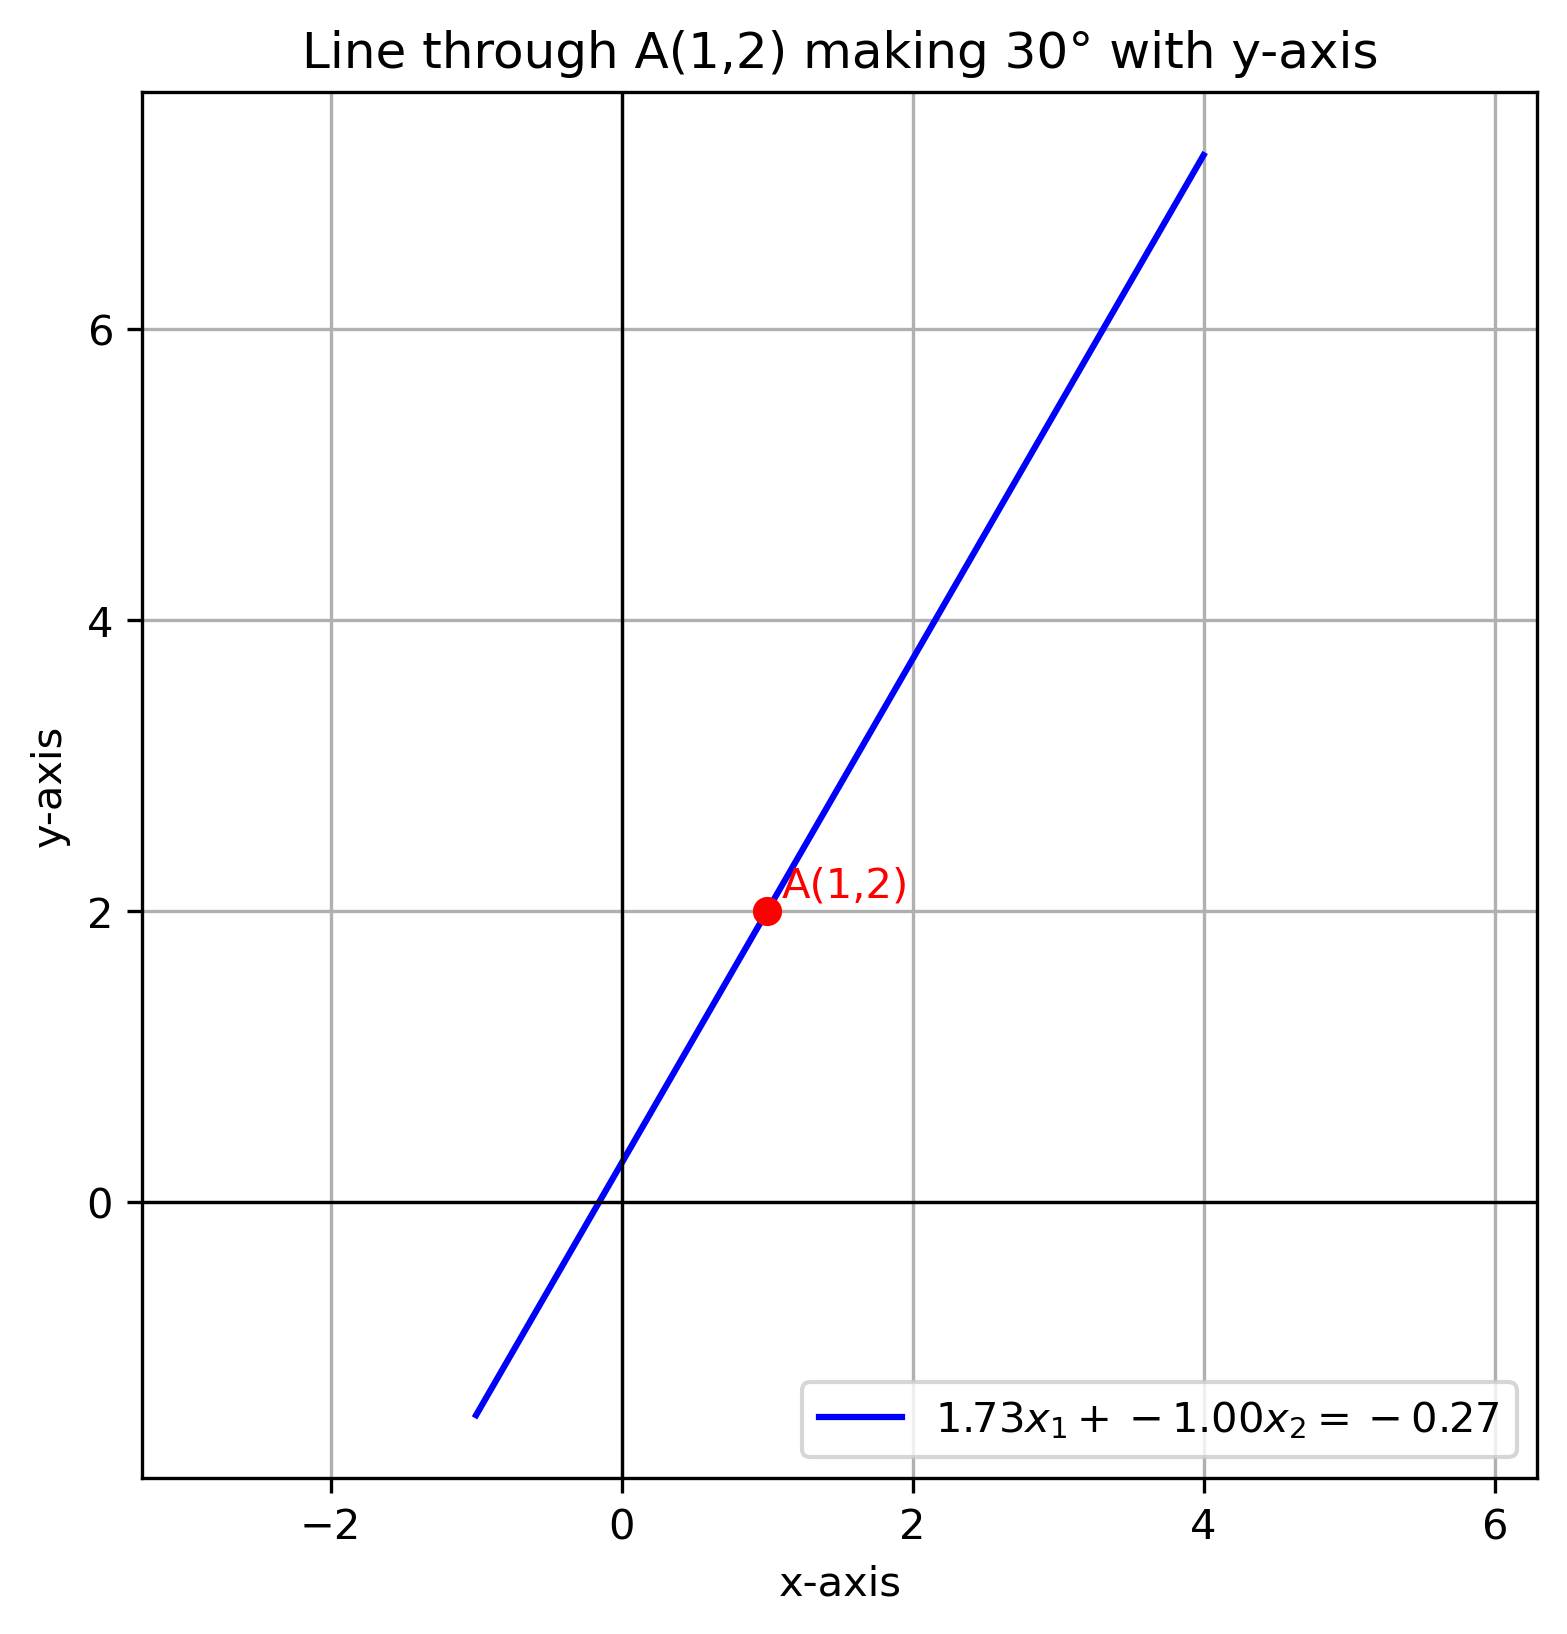
\includegraphics[width=0.7\columnwidth]{figs/fig1.png}
     \caption*{}
     \label{fig:fig1}
 \end{figure}
 
\end{frame}

\end{document}

